\section{Getting at Amp\`ere's law}
\sectionmark{Getting at Ampere's law}
\instructornote{%
By Matt, Fall 2026.  Time: $\sim$30 minutes

include it here in the lab manual for others as well.  


}

\makelabheader %(Space for student name, etc., defined in master.tex)

\bigskip

\textbf{Introduction}

We already know from ideas about electric potential, potential energy, and conservative forces that for a static \textit{electric} field, integrating
$\vv{E} \cdot \vv{ds}$ around a \textit{closed path}%
\footnote{The additional circle in the integral sign $\oint$ emphasizes that the integral is around a \textit{closed} path.}
(or ``loop'') gives
$$\oint \vv{E} \cdot \vv{ds} = 0.$$
In this lab, we ask if the same is true when we integrate the \textit{magnetic} field
$\vv{B} \cdot \vv{ds}$ around a closed loop:
$$\oint \vv{B} \cdot \vv{ds} =~?$$

\begin{wrapfigure}[6]{r}{0.42\textwidth}
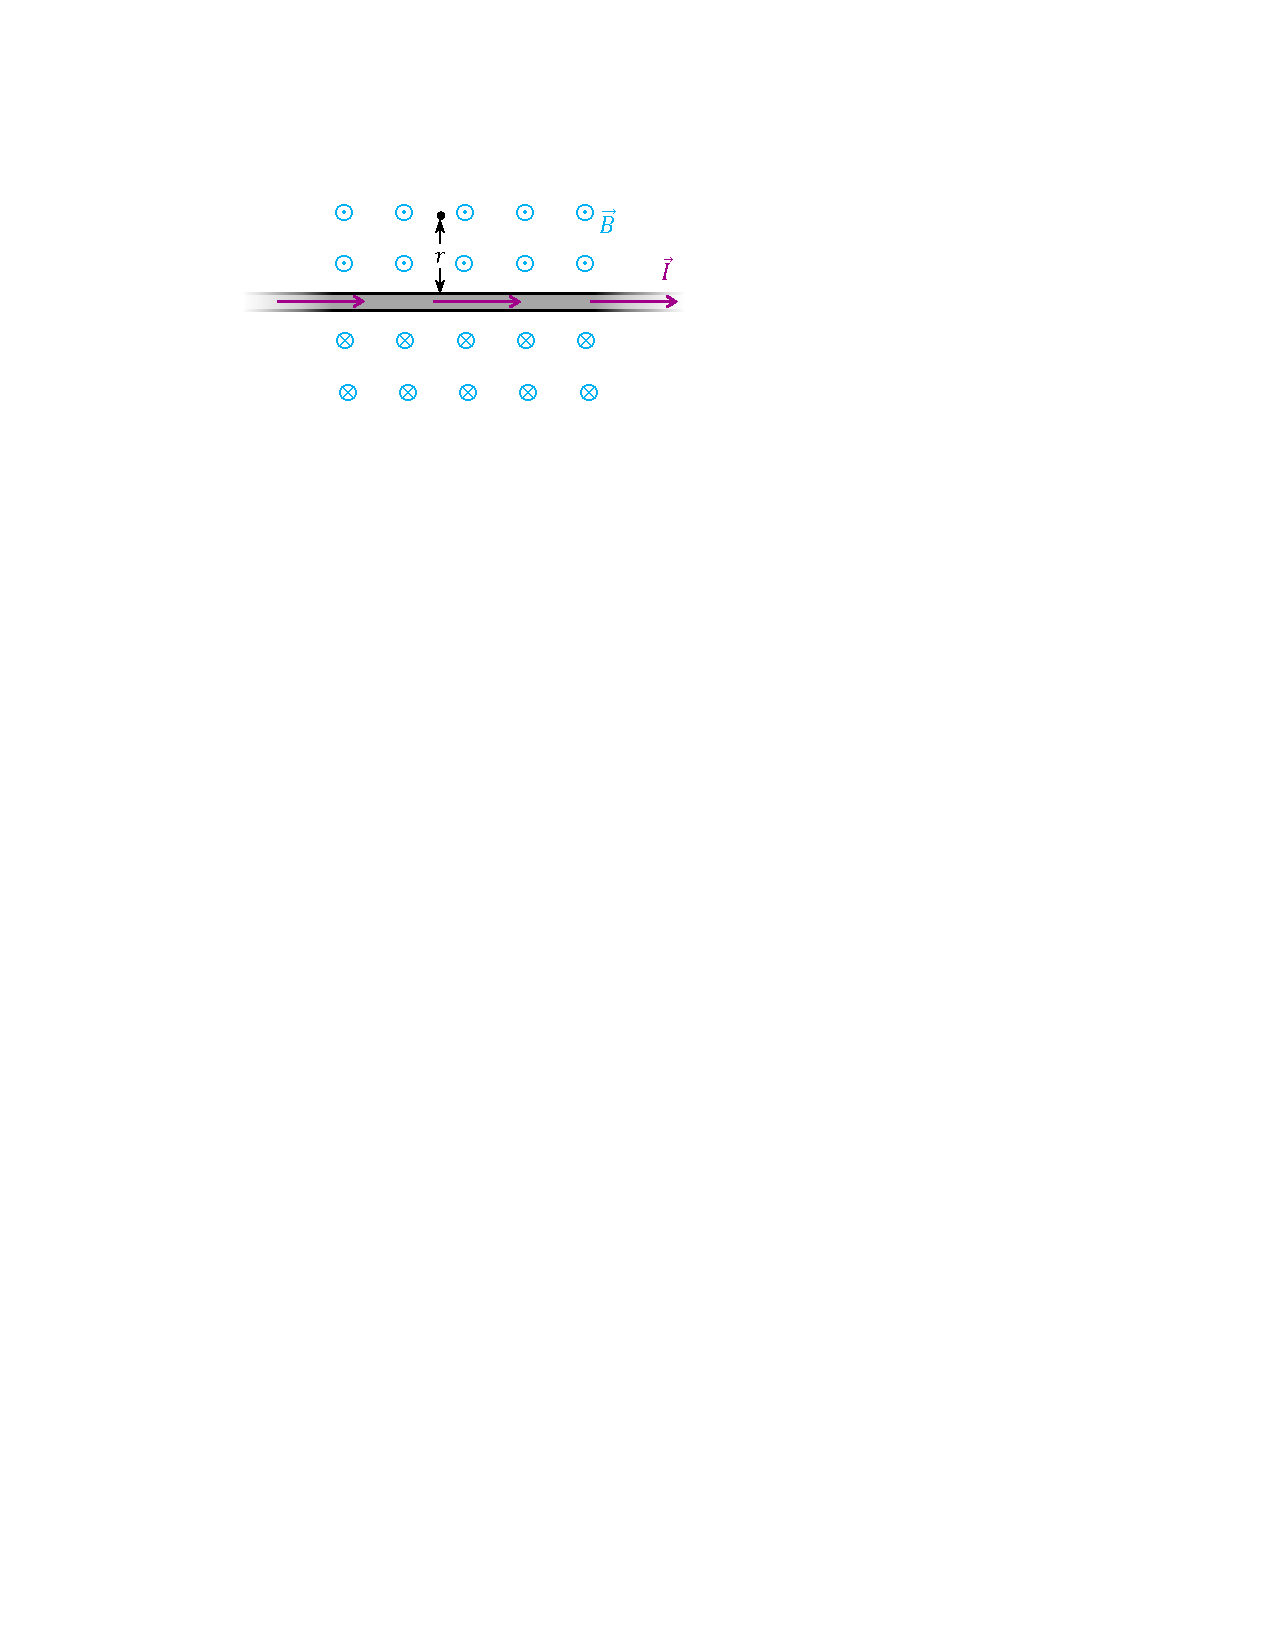
\includegraphics[scale=0.90]{amperes_law_intro/wire_side_view.pdf}
\end{wrapfigure}
\textbf{Activity: Paths Around a Long Straight Wire}

The picture to the right depicts an infinitely long, straight wire carrying a current $I$, which creates a magnetic field circumferentially around the wire given by
$$B=\frac{\mu_0 I}{2 \pi r} ~
\iflabelexists{biot_savart_straight_wire}
	{\text{(from Lab~\ref{biot_savart_straight_wire}, Step 8)}}
	{}
,$$
where $r$ is the distance from the wire.

\begin{enumerate}[labparts]

\item The picture below shows an end-on view of the same straight wire, with current 
$\vv{I}$ coming out of the page.  Calculate the value of $\displaystyle \oint \vv{B} \cdot \vv{ds}$ in a circular path of radius $r$ around the wire. (It's definitely \textit{NOT} zero!)

	\hspace{0.5in}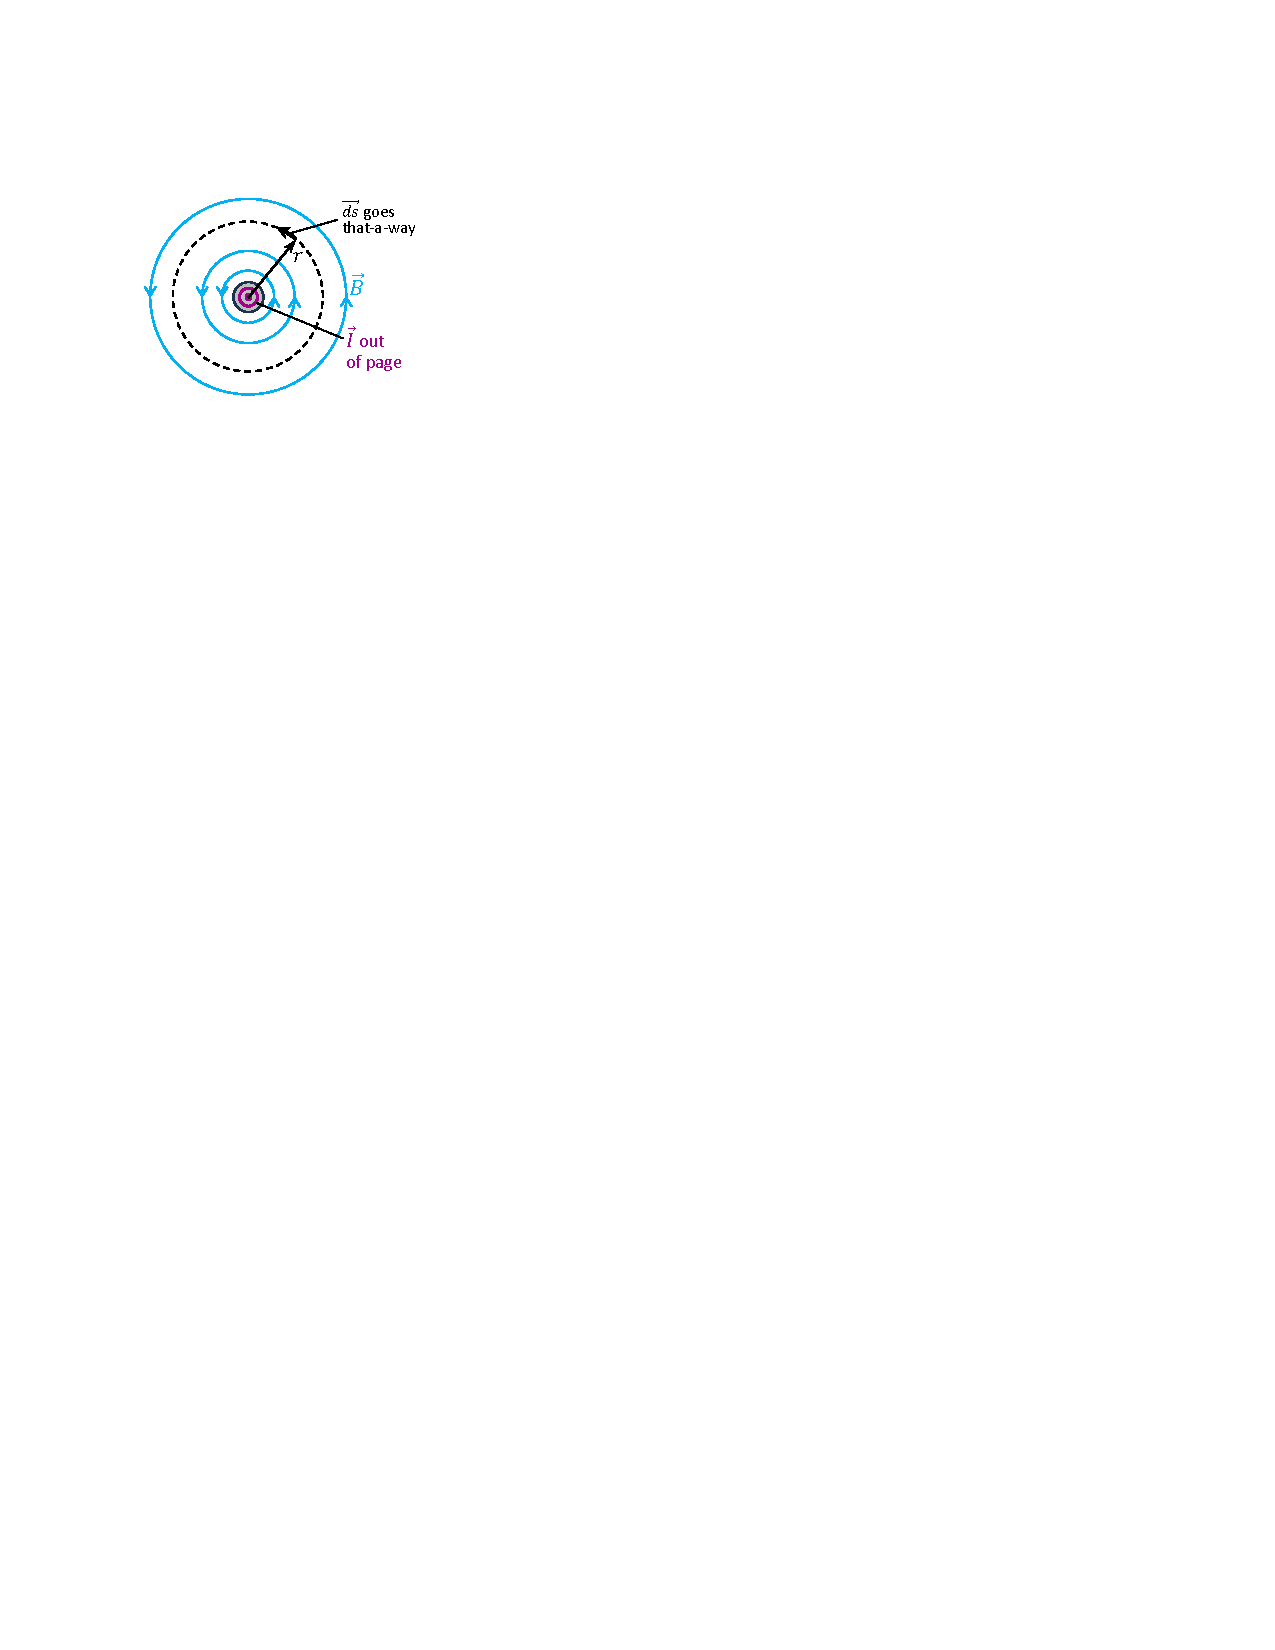
\includegraphics{amperes_law_intro/circular_path.pdf}
	\vspace{-0.1in}

\item What is $\displaystyle \oint \vv{B} \cdot \vv{ds}$ when the path is changed to two semicircles as shown below? Here you'll need to break the integral up into four separate parts.  What is the angle $\theta$ between $\vv{B}$ and $\vv{ds}$ for the two straight segments?

	\hspace{0.5in}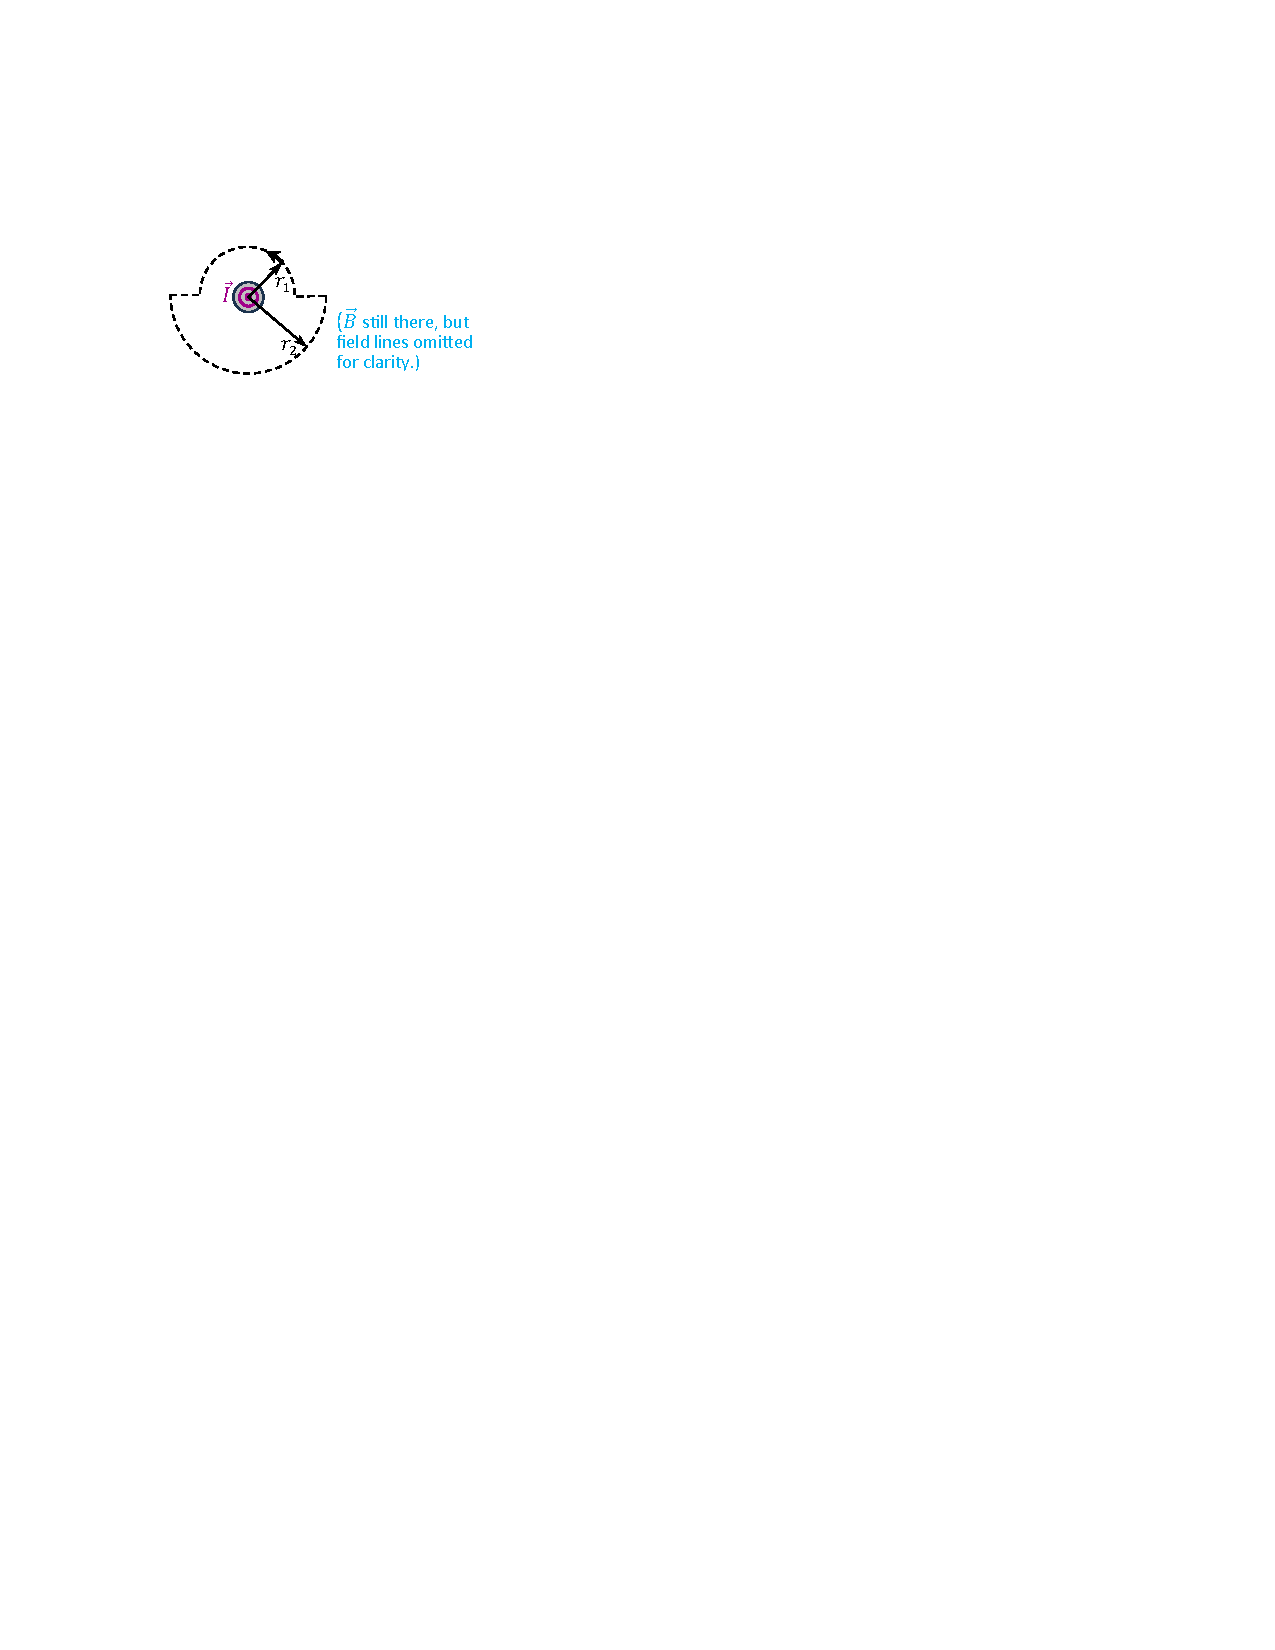
\includegraphics{amperes_law_intro/two_semicircles.pdf}
	\vspace{-0.1in}

\item We can even have four or more curved, circumferential sections, connected by radial straight lines. What's $\displaystyle \oint \vv{B} \cdot \vv{ds}$ in each of these cases?

	\vspace*{-0.1in}
	\hspace*{0.5in}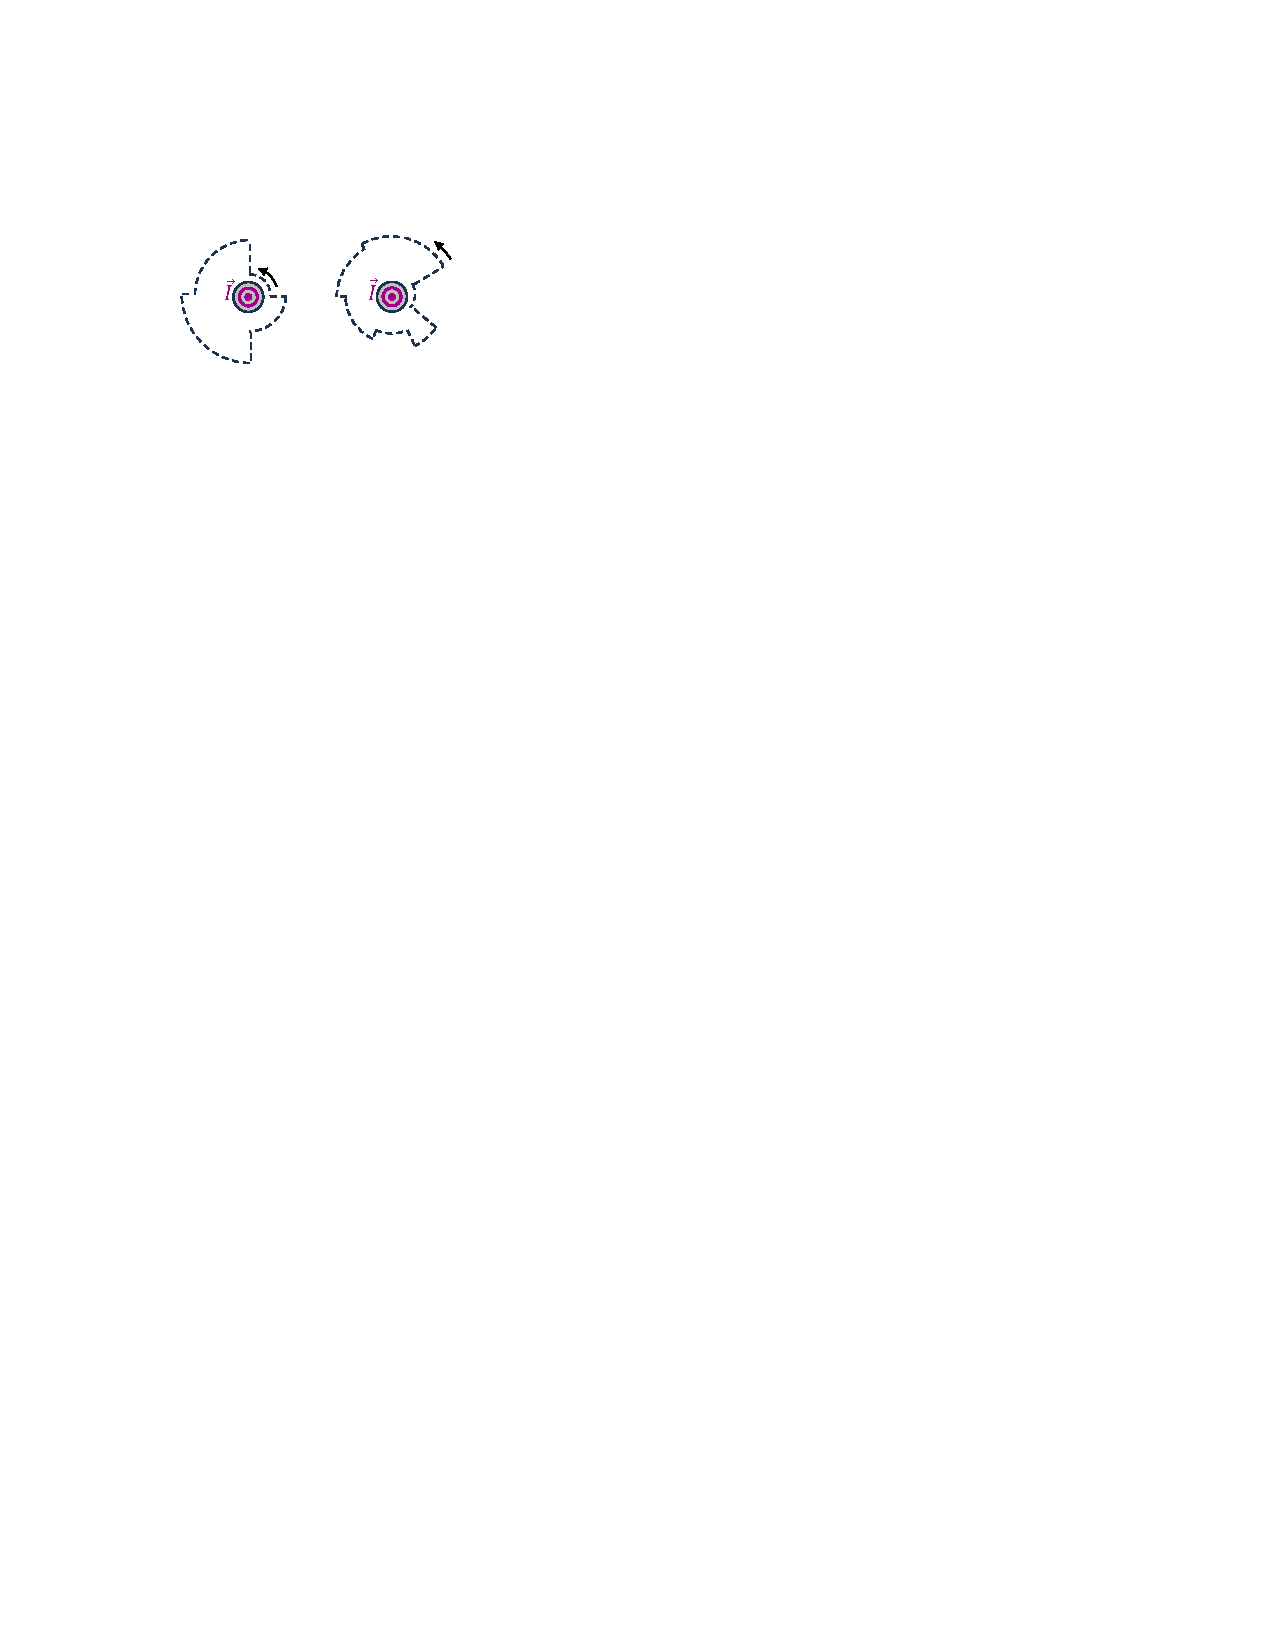
\includegraphics{amperes_law_intro/more_segments.pdf}

\item In fact, you can approximate \textit{any} arbitrary path as a series of infinitesimally small alternating radial and circumferential steps, as shown.  What is $\displaystyle \oint \vv{B} \cdot \vv{ds}$ here? \\
	\hspace*{0.5in}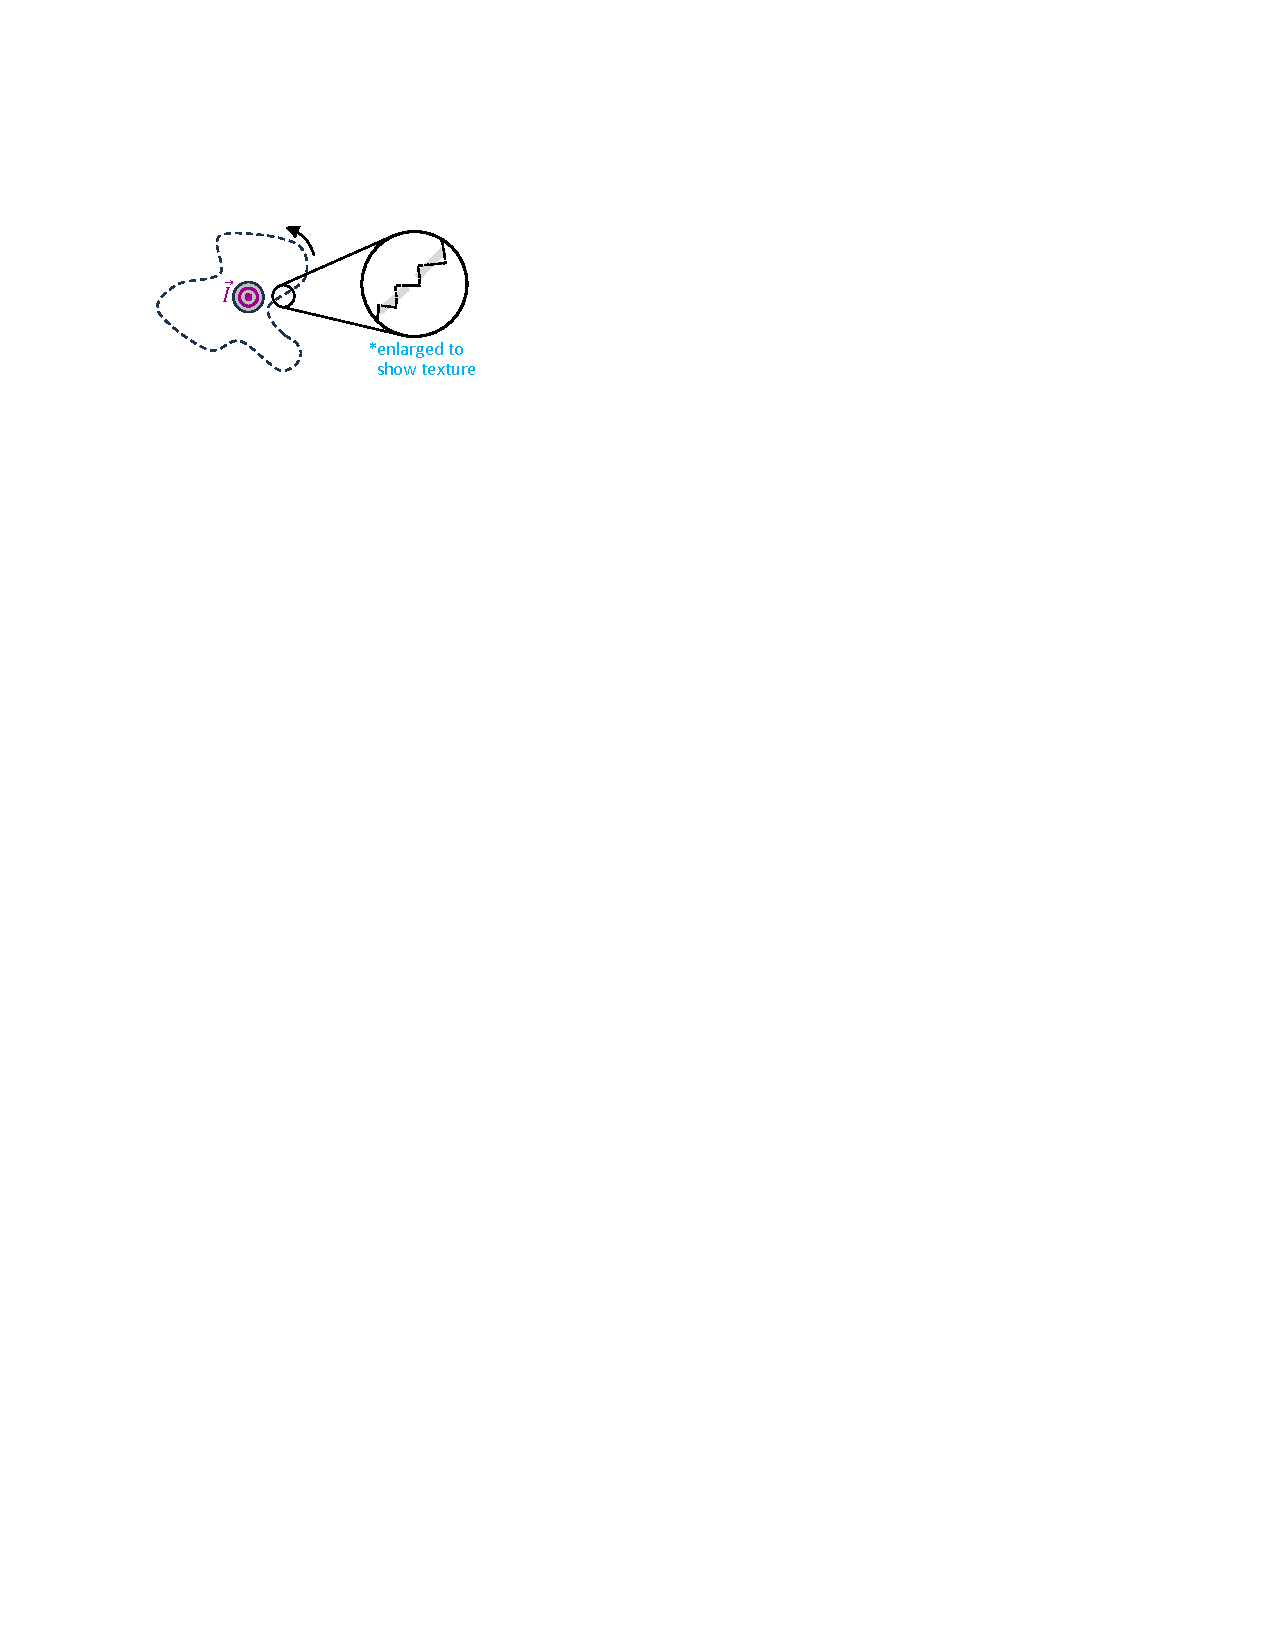
\includegraphics{amperes_law_intro/arbitrary_path.pdf}
	\vspace{-0.1in}
\label{arbitrary_path}

\item In the drawing below, we're back to two semicircles, but now the path doesn't enclose the wire. 
What is the angle $\theta$ between $\vv{B}$ and $\vv{ds}$ in each of the four legs, and what is 
$\displaystyle \oint \vv{B} \cdot \vv{ds}$?  (Be careful with your signs!) \\
	\hspace*{0.5in}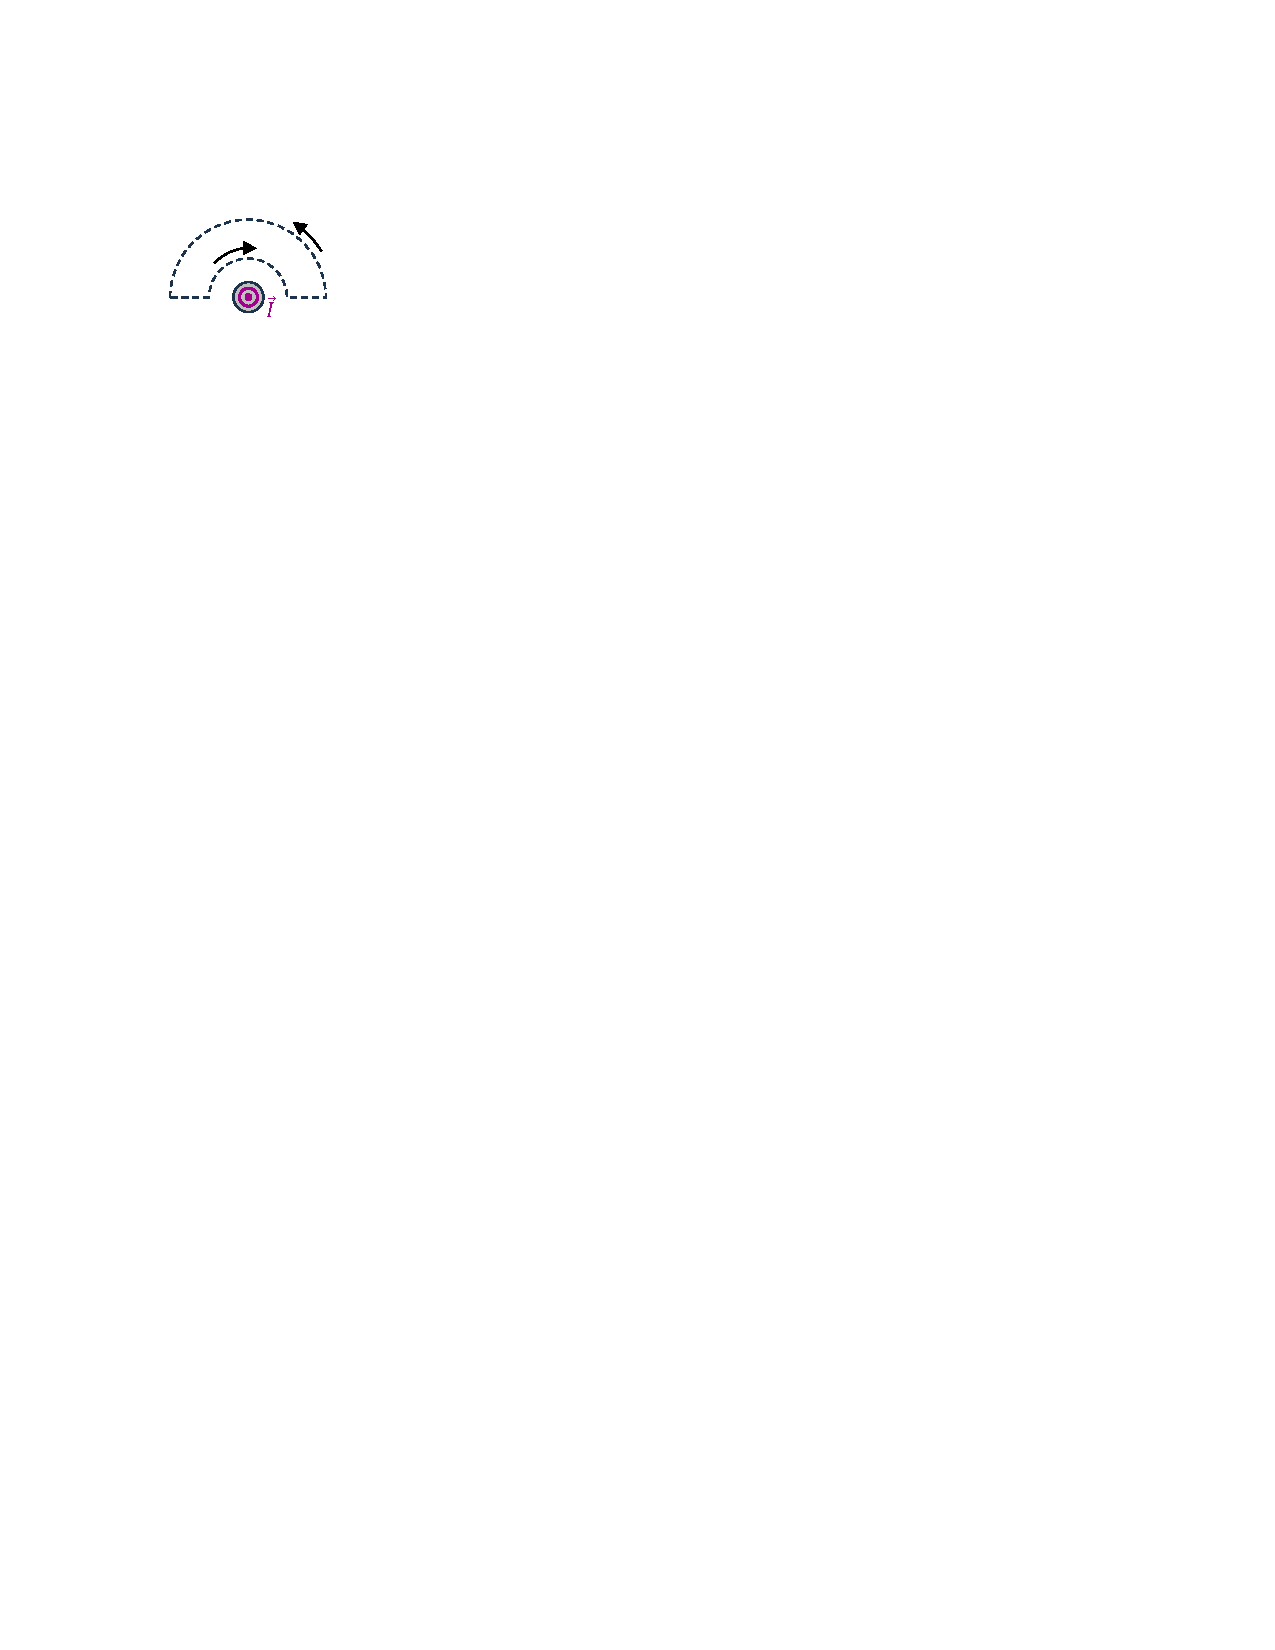
\includegraphics{amperes_law_intro/two_semicircles_zero_enclosed.pdf}
	\vspace{-0.1in}

\item What's $\displaystyle \oint \vv{B} \cdot \vv{ds}$ here?  Does the exact shape of the path make any difference? \\
	\hspace*{0.5in}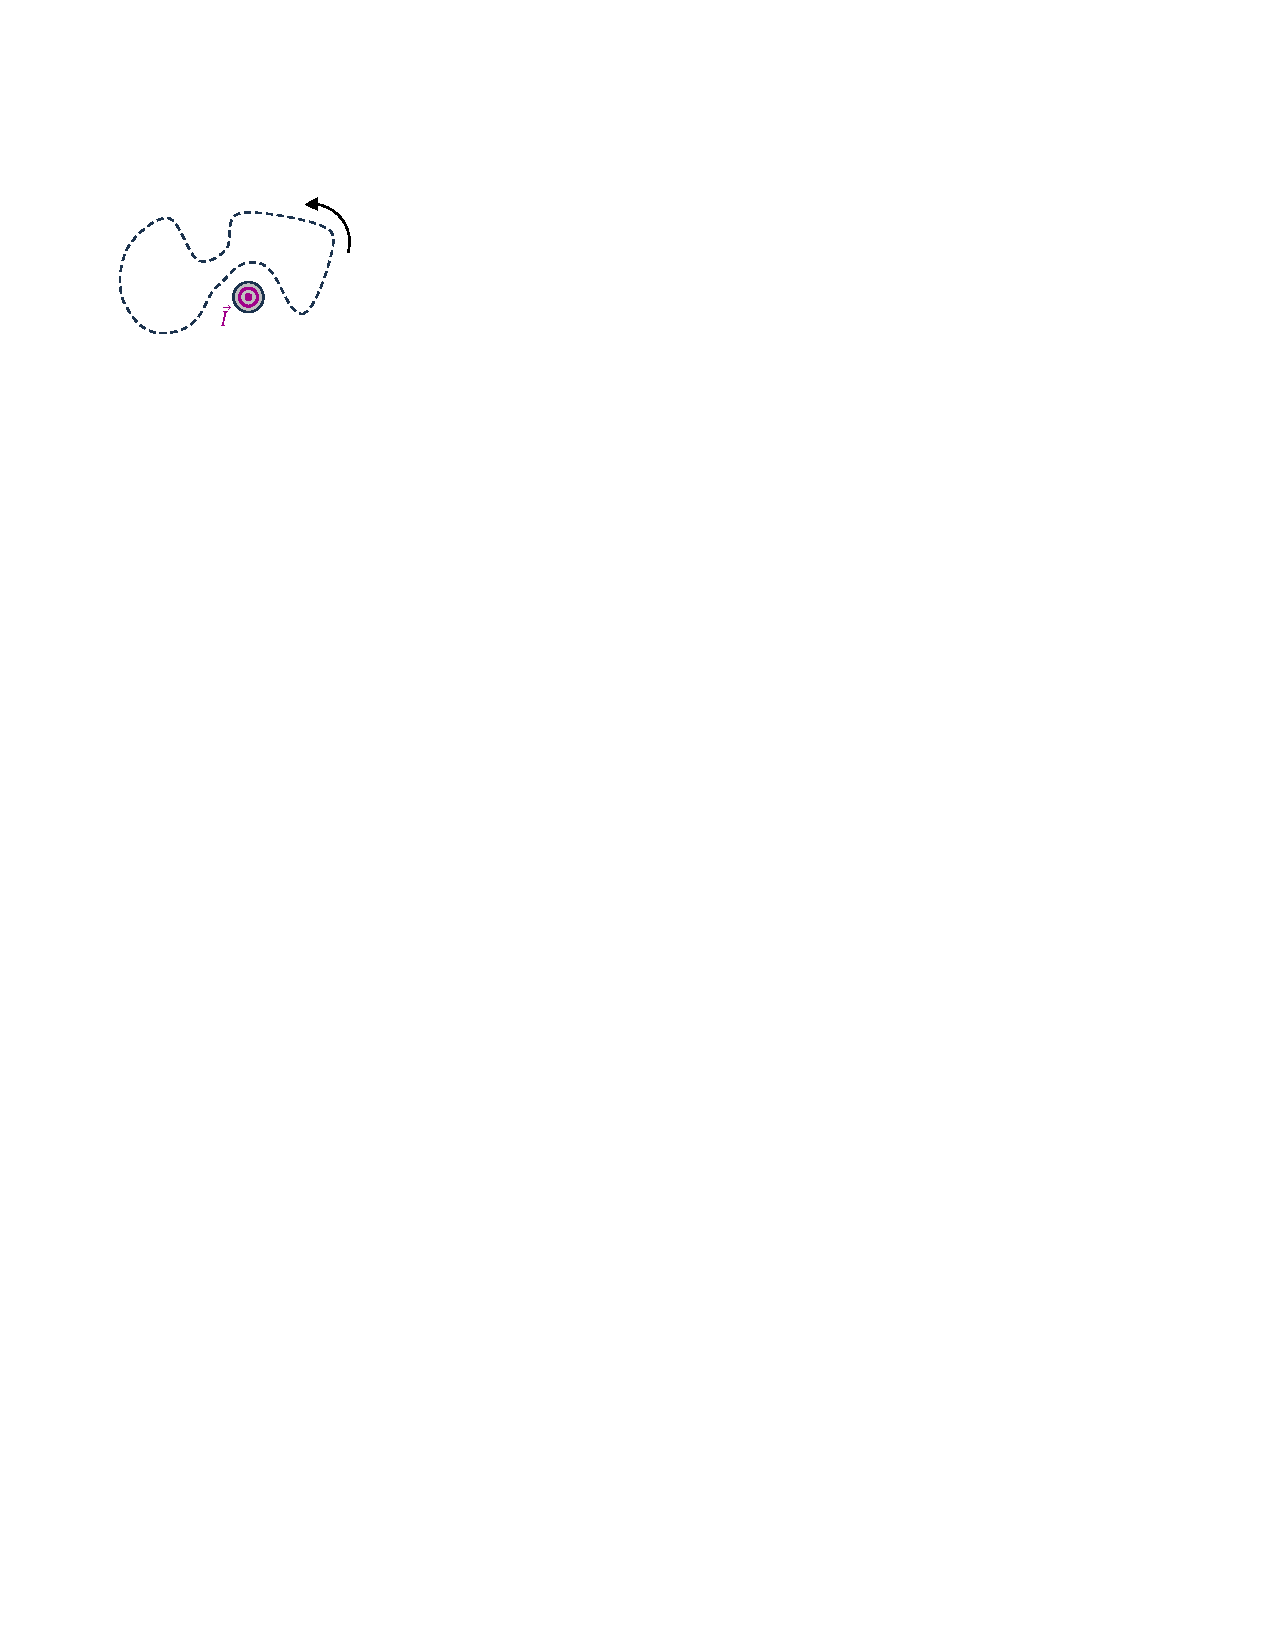
\includegraphics{amperes_law_intro/arbitrary_path_zero_enclosed.pdf}
	\vspace{-0.1in}
\label{arbitrary_path_zero_enclosed}

\item It seems like the key difference between parts \ref{arbitrary_path} 
and \ref{arbitrary_path_zero_enclosed} 
is whether the loop \textit{encloses} a wire with current.  What is $\displaystyle \oint \vv{B} \cdot \vv{ds}$ if the loop encloses two wires with different currents $I_1$ and $I_2$? 
(Hint: $\vv{B}_\text{net} = \vv{B}_{I_1} + \vv{B}_{I_2}$, yes?)\\
	\hspace*{0.5in}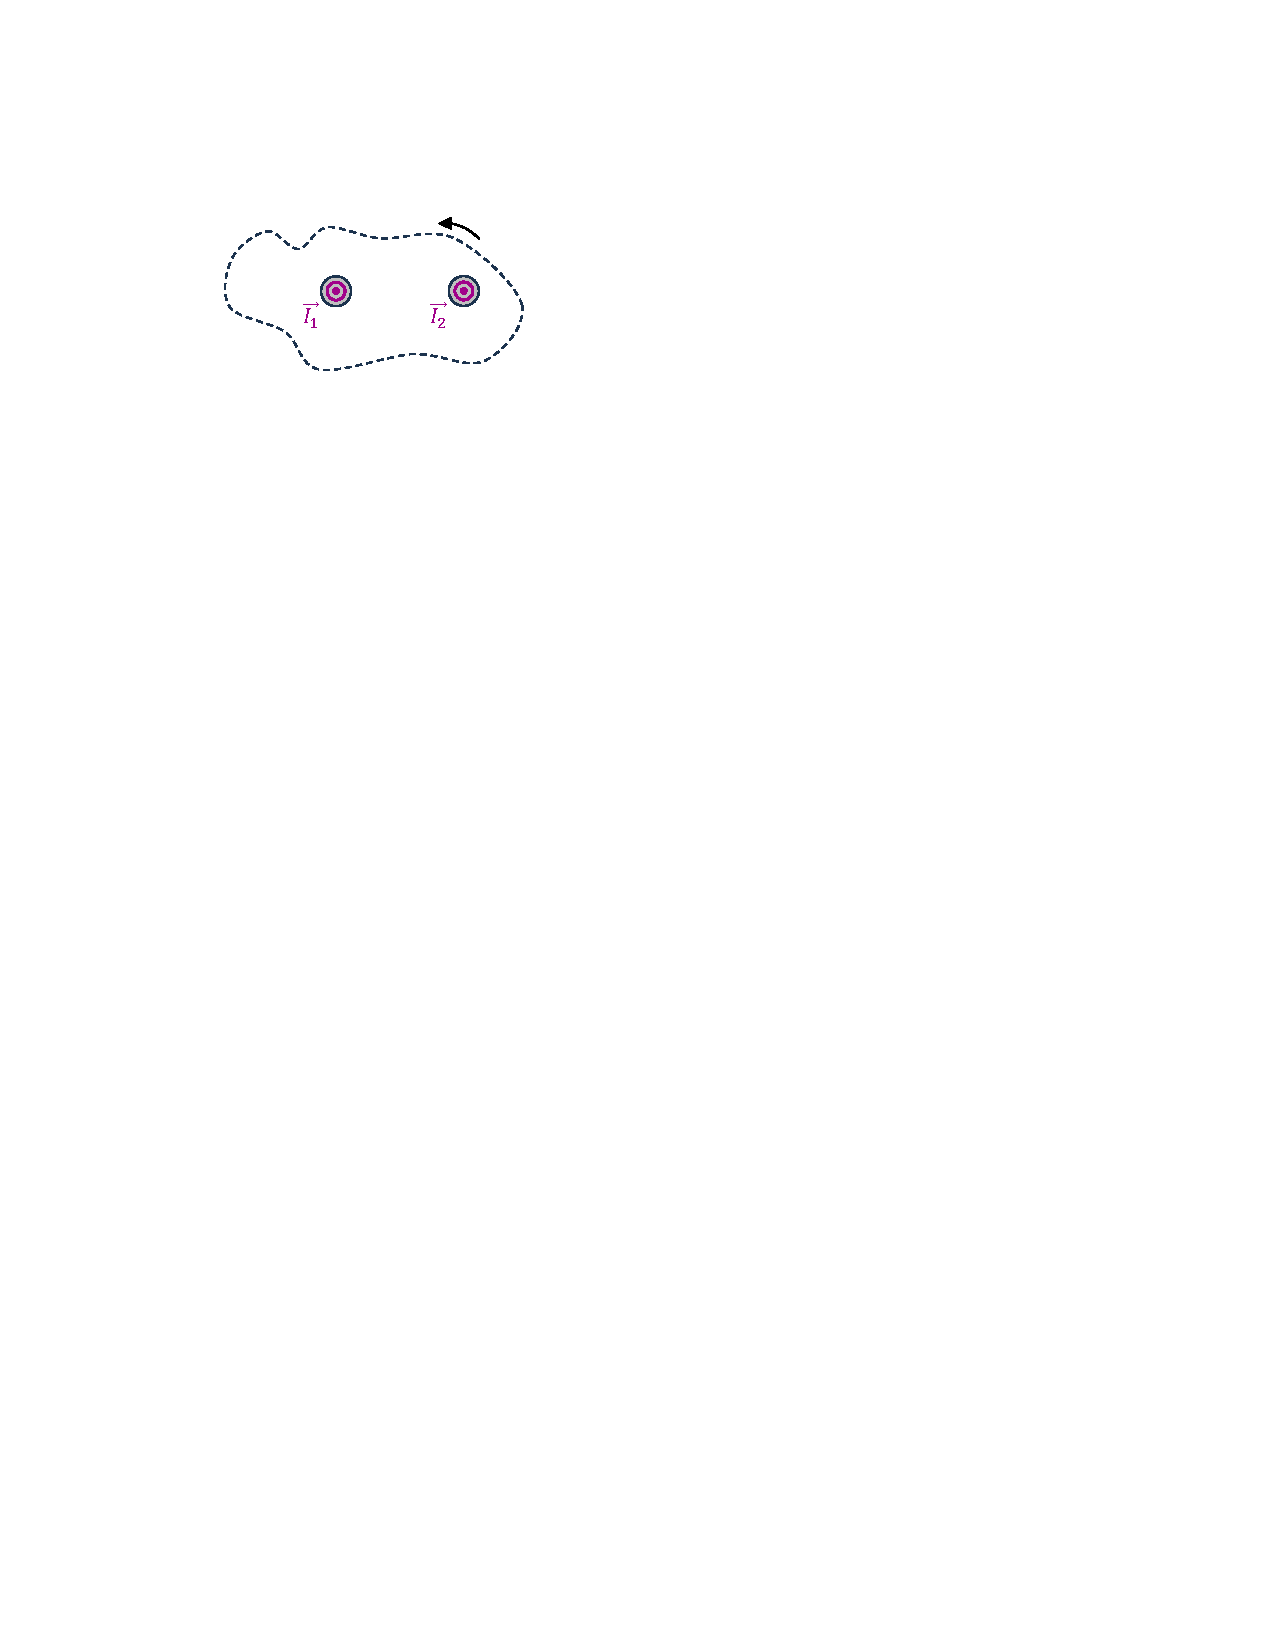
\includegraphics{amperes_law_intro/two_wires.pdf}
	\vspace*{-0.1in}

\item What if the two enclosed wires have equal current but in opposite directions?  Now what's $\displaystyle \oint \vv{B} \cdot \vv{ds}$? \\
	\hspace*{0.5in}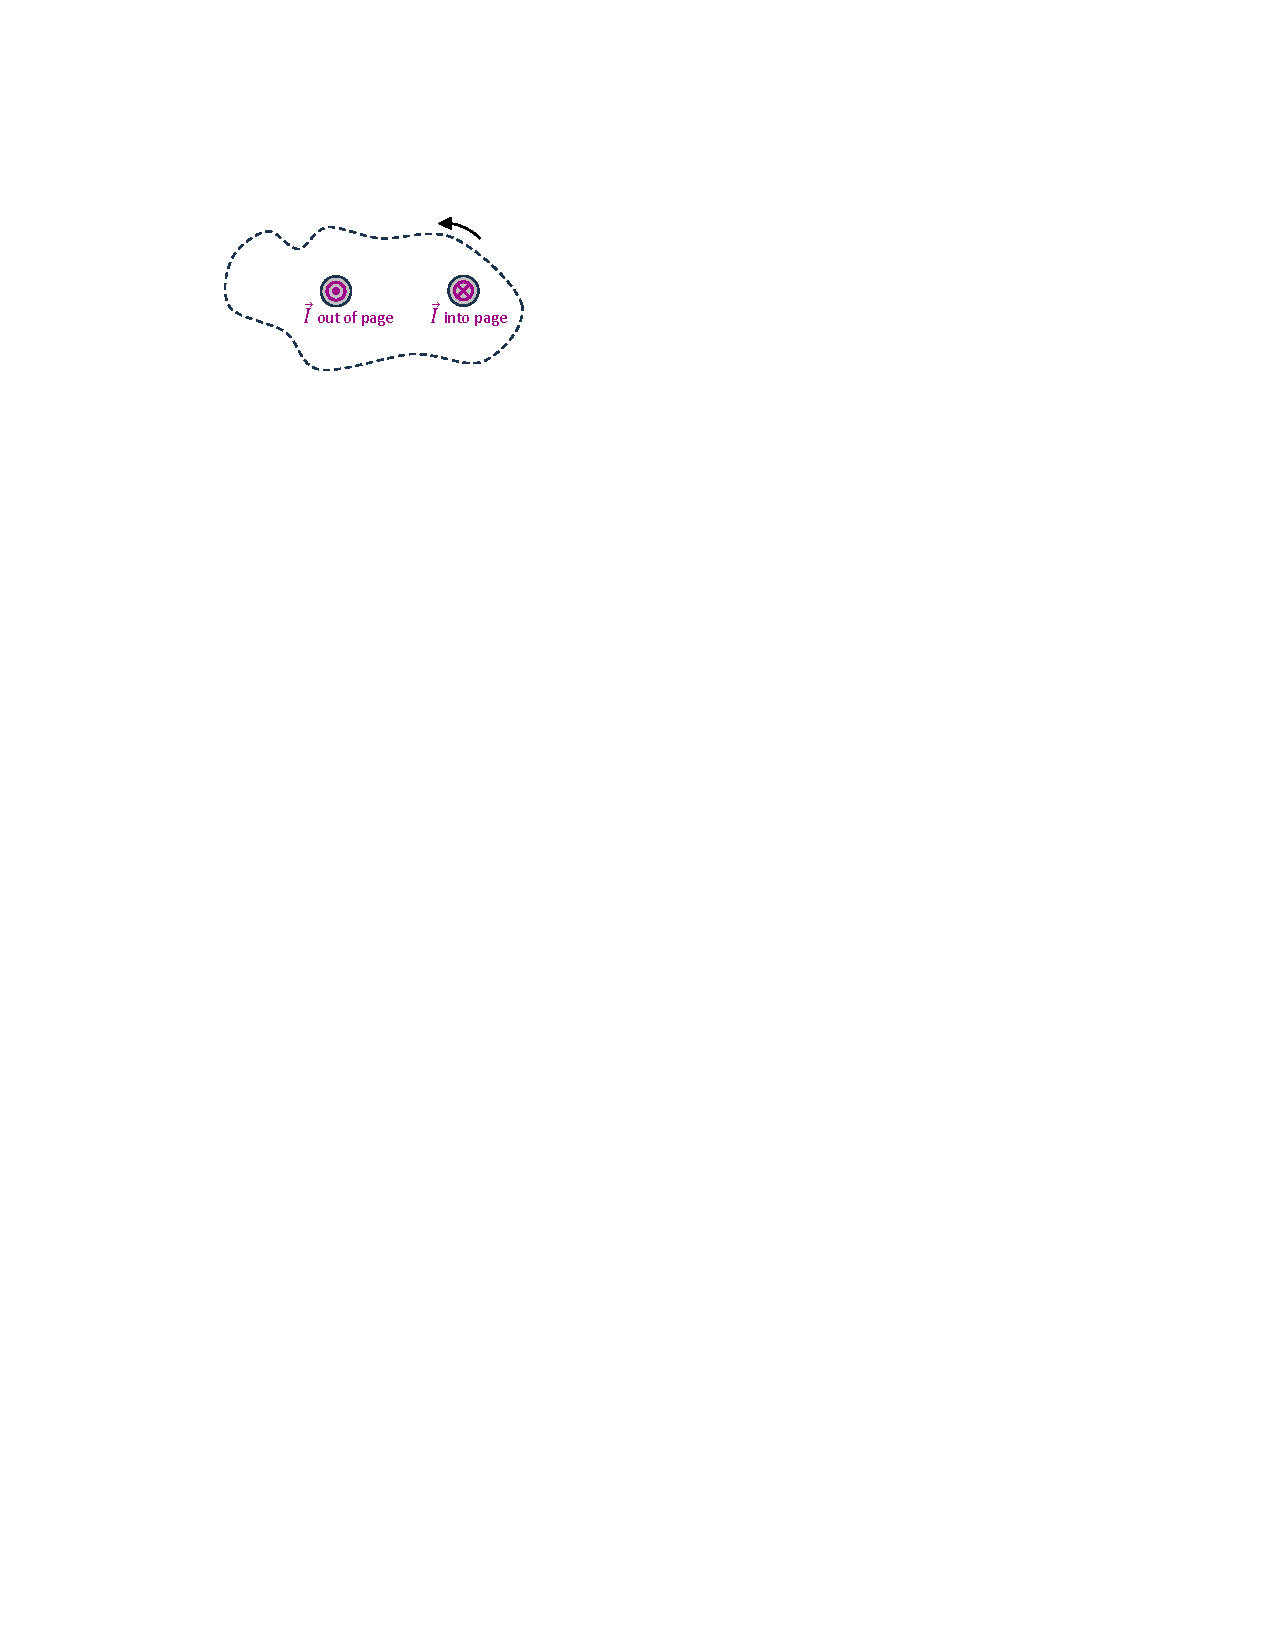
\includegraphics{amperes_law_intro/two_wires_zero_enclosed.pdf}
	\vspace*{-0.1in}

\item Our friend Mr. Amp\`ere is stuck!
Can you help him write a general law
that relates the integral $\displaystyle \oint \vv{B} \cdot \vv{ds}$ around a closed path to the total enclosed%
\footnote{Technically, you've only seen that this relationship holds for the special case of infinitely long, straight wires.  But it turns out that it's also true for wires of any shape whatsoever.}
current $I_\text{enc}$ within the path?
Amp\`ere thanks you!  :-)

\answerspace{\fill}

\end{enumerate}
